% 行间 · AI 旅行规划 Agent —— 技术文档
% 编译：在 docs/latex 目录执行 latexmk -xelatex technical-doc.tex（或 npm run docs:pdf）
\documentclass[a4paper]{article}

% ---------- 页面与字体 ----------
\usepackage[a4paper,top=2.4cm,bottom=2.3cm,left=2.3cm,right=2.3cm,headheight=20pt]{geometry}
\usepackage{fontspec}
\usepackage{xeCJK}
\setmainfont{Libertinus Serif}
\setsansfont{Libertinus Sans}
\setmonofont{Consolas}[Scale=0.9]
\setCJKmainfont{NotoSerifCJKsc-Regular.otf}[BoldFont=NotoSerifCJKsc-Bold.otf]
\setCJKsansfont{SourceHanSansCN-Regular.otf}
\setCJKmonofont{SourceHanSansCN-Regular.otf}
\newCJKfontfamily\heavyfont{NotoSerifCJKsc-Black.otf}
\xeCJKsetup{CJKspace=false}
\linespread{1.35}
\setlength{\parindent}{2em}
\setlength{\parskip}{3pt}
\setlength{\emergencystretch}{3em}
\renewcommand{\contentsname}{目录}
\renewcommand{\figurename}{图}
\renewcommand{\tablename}{表}

% ---------- 宏包 ----------
\usepackage{xcolor}
\usepackage{graphicx}
\graphicspath{{../}}
\usepackage{longtable,booktabs,array,colortbl,calc}
\usepackage{caption}
\usepackage{float}
\usepackage{enumitem}
\usepackage{titlesec,titletoc}
\usepackage{fancyhdr}
\usepackage{fancyvrb}
\usepackage[most]{tcolorbox}
\usepackage{tikz}
\usetikzlibrary{arrows.meta,positioning,calc,shapes.misc,fit,backgrounds}
\usepackage[hidelinks,bookmarksnumbered]{hyperref}
\hypersetup{pdftitle={行间 · AI 旅行规划 Agent 技术文档},pdfauthor={行间团队}}

% ---------- 配色（与产品一致：暖纸、墨色、松绿） ----------
\definecolor{ink}{HTML}{1D1914}
\definecolor{inksoft}{HTML}{5C5348}
\definecolor{inkfaint}{HTML}{8D8274}
\definecolor{pine}{HTML}{1F5A47}
\definecolor{pinesoft}{HTML}{DBE8E0}
\definecolor{paper}{HTML}{F6F1E7}
\definecolor{paperdeep}{HTML}{ECE4D4}
\definecolor{line}{HTML}{DDD2BF}
\definecolor{clay}{HTML}{B0512A}
\definecolor{sky}{HTML}{2D5B78}
\definecolor{skysoft}{HTML}{DDE8EF}
\color{ink}

% ---------- 标题样式 ----------
\titleformat{\section}[block]
  {\Large\bfseries\color{ink}}
  {\color{pine}\heavyfont\thesection}{0.8em}{}
  [\vspace{2pt}{\color{ink}\titlerule[0.8pt]}]
\titlespacing*{\section}{0pt}{22pt}{12pt}
\titleformat{\subsection}
  {\large\bfseries\color{pine}}{\thesubsection}{0.7em}{}
\titlespacing*{\subsection}{0pt}{14pt}{6pt}
% 章节之间不强制换页；放宽浮动参数，减少图片造成的留白
\renewcommand{\topfraction}{0.85}
\renewcommand{\bottomfraction}{0.7}
\renewcommand{\textfraction}{0.1}
\renewcommand{\floatpagefraction}{0.75}
\setcounter{topnumber}{3}
\setcounter{bottomnumber}{2}
\setcounter{totalnumber}{4}

\titlecontents{section}[0pt]{\addvspace{4pt}\bfseries}
  {\thecontentslabel\quad}{}{\hfill\contentspage}
\titlecontents{subsection}[2.2em]{\small\color{inksoft}}
  {\thecontentslabel\quad}{}{\titlerule*[0.6pc]{.}\contentspage}

% ---------- 页眉页脚 ----------
\pagestyle{fancy}
\fancyhf{}
\fancyhead[L]{\small\color{inkfaint}行间 · AI 旅行规划 Agent 技术文档}
\fancyhead[R]{\small\color{inkfaint}\leftmark}
\fancyfoot[C]{\small\color{inkfaint}\thepage}
\renewcommand{\headrulewidth}{0.4pt}
\renewcommand{\headrule}{\hbox to\headwidth{\color{line}\leaders\hrule height \headrulewidth\hfill}}
\renewcommand{\sectionmark}[1]{\markboth{\thesection\quad #1}{}}

% ---------- 列表 ----------
\setlist{nosep,leftmargin=2em,itemsep=2pt,topsep=4pt}
\setlist[itemize]{label=\textcolor{pine}{\small\textbullet}}

% ---------- 图 ----------
\captionsetup{font={small,color=inksoft},labelfont=bf,labelsep=quad,skip=5pt}
\newcommand{\shot}[2][height=0.3\textheight]{%
  \begin{tikzpicture}
    \node[inner sep=0pt] (img) {\includegraphics[width=\linewidth,#1,keepaspectratio]{#2}};
    \draw[line,line width=0.6pt,rounded corners=2pt] (img.south west) rectangle (img.north east);
  \end{tikzpicture}}

% ---------- 表（三线表，表头底色） ----------
\newcommand{\thead}[1]{\textbf{#1}}
\newenvironment{doctable}[1]
  {\par\small\renewcommand{\arraystretch}{1.35}\setlength{\LTpre}{6pt}\setlength{\LTpost}{8pt}%
   \begin{longtable}{#1}\toprule\rowcolor{paperdeep}}
  {\bottomrule\end{longtable}}

% ---------- 代码 ----------
\newcommand{\code}[1]{\texttt{\textcolor{pine}{#1}}}
\newtcblisting{codeblock}{listing only,breakable,colback=paper,colframe=line,boxrule=0.5pt,arc=2pt,
  left=8pt,right=8pt,top=3pt,bottom=3pt,
  listing options={basicstyle=\small\ttfamily,columns=fullflexible,keepspaces=true,breaklines=true,extendedchars=true}}

% pandoc 生成内容所需的兼容命令
\providecommand{\tightlist}{}
\providecommand{\passthrough}[1]{#1}
\def\labelenumi{\arabic{enumi}.}

% ---------- 图示：系统架构 ----------
\tikzset{
  layer/.style={draw=pine,fill=paper,rounded corners=4pt,line width=0.8pt,text width=#1,inner sep=7pt,align=left,font=\small},
  module/.style={draw=sky,fill=skysoft!55,rounded corners=4pt,line width=0.7pt,text width=#1,inner sep=6pt,align=left,font=\small,minimum height=1.55cm},
  flowbox/.style={draw=pine,fill=paper,rounded corners=3pt,line width=0.7pt,font=\footnotesize\ttfamily,align=center,inner sep=4pt,minimum height=1.05cm,text width=2.55cm},
  link/.style={-{Stealth[length=5pt]},line width=0.7pt,color=inkfaint},
}
\newcommand{\layertitle}[1]{{\bfseries\color{pine}#1}\\[1pt]}
\newcommand{\moduletitle}[1]{{\bfseries\color{sky}#1}\\[1pt]}

\newcommand{\ArchitectureDiagram}{%
\begin{figure}[htbp]\centering
\begin{tikzpicture}[node distance=7mm]
  \node[layer=0.94\linewidth] (ui) {\layertitle{浏览器 · React 19 / Next.js App Router}
    {\color{inksoft}首页滚动叙事 · 需求表单（语音、照片） · 规划轨迹 · 旅行手册 · 地图 · 对话栏（调整 / 问答） · 分享长图\\
    Zustand + localStorage：行程、版本历史、规划轨迹、问答记录}};
  \node[layer=0.94\linewidth,below=of ui] (api) {\layertitle{Next.js Route Handlers}
    {\color{inksoft}/api/agent（规划 / 调整） · /api/ask（问答） · /api/reschedule（手动重排） · /api/vision（照片识景） · /api/photo（图片代理） · /\_AMapService（地图安全代理）\\
    同源校验 · Zod 输入校验 · 限流与并发控制 · 错误映射}};
  \draw[link] (ui) -- node[right,font=\scriptsize,color=inkfaint]{同源 HTTP · NDJSON 流} (api);
  \node[module=0.285\linewidth,below=8mm of api.south west,anchor=north west] (agent) {\moduletitle{规划 Agent}ReAct 主循环 · 工具调用 · 校验反馈};
  \node[module=0.285\linewidth,right=3.2mm of agent] (ask) {\moduletitle{问答 Agent}只读工具子集 · 来源标注};
  \node[module=0.285\linewidth,right=3.2mm of ask] (engine) {\moduletitle{确定性引擎}空间聚类 · 路径排序 · 排程器 · 预算};
  \draw[link] (api.south -| ask.north) -- node[right,font=\scriptsize,color=inkfaint]{编排} (ask.north);
  \node[module=0.205\linewidth,below=8mm of agent.south west,anchor=north west] (llm) {\moduletitle{大模型}DeepSeek-V4.1-Flash（文本与图片）};
  \node[module=0.205\linewidth,right=3mm of llm] (amap) {\moduletitle{高德开放平台}POI · 周边 · 路线 · 跨城铁路 · 天气};
  \node[module=0.205\linewidth,right=3mm of amap] (rag) {\moduletitle{知识库 RAG}47 篇目的地知识 · BM25};
  \node[module=0.205\linewidth,right=3mm of rag] (opt) {\moduletitle{可选服务}Tavily 联网搜索};
  \draw[link] (agent.south) -- ++(0,-4mm) -| (llm.north);
  \draw[link] (ask.south) -- ++(0,-4mm) -| (amap.north);
  \draw[link] (engine.south) -- ++(0,-4mm) -| (rag.north);
  \draw[link] (engine.south) -- ++(0,-4mm) -| (opt.north);
\end{tikzpicture}
\caption{系统总体架构}
\end{figure}}

% ---------- 图示：Agent 工作流 ----------
\newcommand{\AgentFlowDiagram}{%
\begin{figure}[htbp]\centering
\begin{tikzpicture}[node distance=5mm and 5mm]
  \node[flowbox,font=\footnotesize] (a) {理解需求};
  \node[flowbox,right=of a] (b) {search\_trains\\set\_trains};
  \node[flowbox,right=of b] (c) {search\_knowledge\\get\_weather};
  \node[flowbox,right=of c] (d) {search\_places\\{\rmfamily\scriptsize（并行多关键词）}};
  \node[flowbox,below=9mm of d] (e) {arrange\_places\\set\_hotel};
  \node[flowbox,left=of e] (f) {search\_nearby\\verify\_ticket};
  \node[flowbox,left=of f,draw=clay,fill=clay!8,line width=1pt] (g) {save\_day\_plan\\{\rmfamily\scriptsize（校验 / 排程）}};
  \node[flowbox,left=of g,fill=pinesoft] (h) {finalize\_trip};
  \draw[link] (a) -- (b); \draw[link] (b) -- (c); \draw[link] (c) -- (d);
  \draw[link] (d) -- (e); \draw[link] (e) -- (f); \draw[link] (f) -- (g); \draw[link] (g) -- (h);
  \draw[link,color=clay] (g.south) to[out=-60,in=-120,looseness=5] node[below,font=\scriptsize,color=clay]{冲突回传 → 调整后重提（每天最多 3 次）} (g.south east);
\end{tikzpicture}
\caption{规划 Agent 工作流（服务端校验驱动的自我修正闭环）}
\end{figure}}

\begin{document}

% ---------- 封面 ----------
% 图片：public/images/destinations/hangzhou.jpg（西湖三潭印月），与产品首页同源
\newcommand{\coverfield}[2]{%
  \begin{minipage}[t]{0.47\linewidth}
    {\scriptsize\color{inkfaint}#1}\par\vspace{1pt}
    {\small\color{ink}#2}
  \end{minipage}}
\begin{titlepage}
\thispagestyle{empty}
\setlength{\parindent}{0pt}
\begin{tikzpicture}[remember picture,overlay]
  % 底色
  \fill[paper] (current page.south west) rectangle (current page.north east);
  % 满版照片（上半页）
  \begin{scope}
    \clip (current page.north west) rectangle ([yshift=-13.2cm]current page.north east);
    \node[anchor=center,inner sep=0pt] at ([yshift=-6.6cm]current page.north)
      {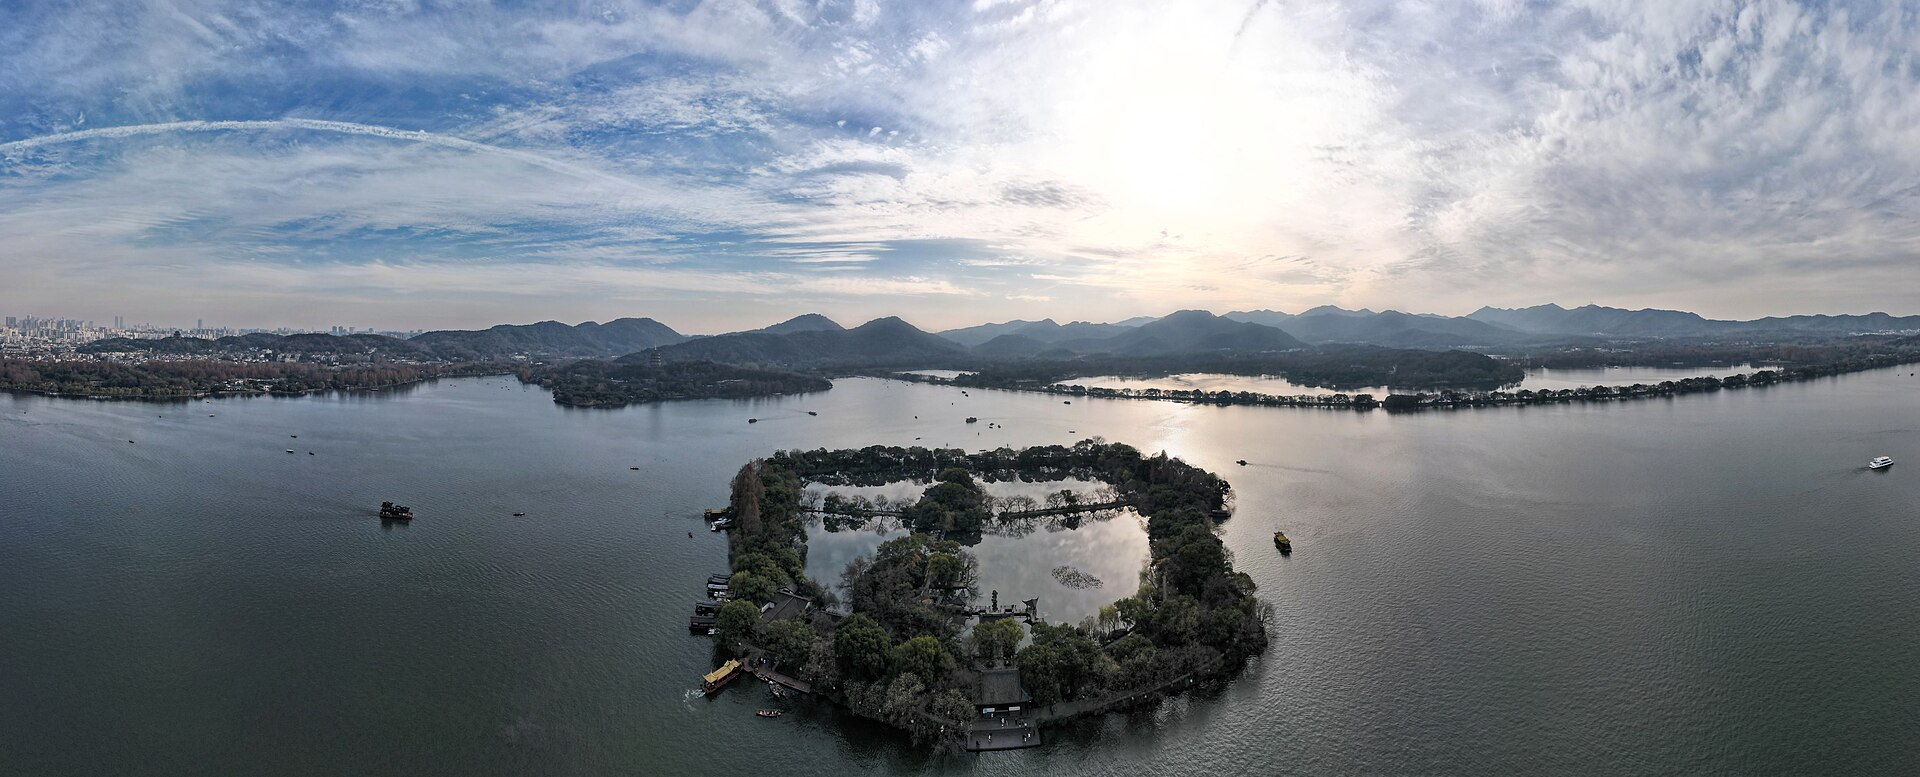
\includegraphics[height=13.4cm]{../public/images/destinations/hangzhou.jpg}};
  \end{scope}
  % 照片顶部压暗一条，承托刊名
  \fill[black,opacity=0.28] (current page.north west) rectangle ([yshift=-1.9cm]current page.north east);
  \node[anchor=west,text=white,font=\large\heavyfont] at ([xshift=2.3cm,yshift=-0.95cm]current page.north west) {行间};
  \node[anchor=east,text=white,font=\footnotesize] at ([xshift=-2.3cm,yshift=-0.95cm]current page.north east)
    {第九届“传智杯”AI Web 网页开发挑战赛};
  % 照片图注
  \node[anchor=south east,text=white,font=\scriptsize,fill=black,fill opacity=0.35,text opacity=1,inner sep=4pt]
    at ([xshift=-2.3cm,yshift=-12.85cm]current page.north east) {杭州 · 西湖三潭印月};
  % 照片下沿的松绿细条
  \fill[pine] ([yshift=-13.2cm]current page.north west) rectangle ([yshift=-13.45cm]current page.north east);
  % 页面底部
  \fill[pine] (current page.south west) rectangle ([yshift=0.35cm]current page.south east);
\end{tikzpicture}

\vspace*{11.25cm}
{\footnotesize\color{pine}\bfseries 技 术 文 档\quad\textcolor{line}{|}\quad\mdseries TECHNICAL DOCUMENTATION}\par
\vspace{0.55cm}
{\fontsize{52}{58}\selectfont\heavyfont 行间}\par
\vspace{0.25cm}
{\fontsize{22}{28}\selectfont\heavyfont AI 旅行规划 Agent}\par
\vspace{0.45cm}
{\large\color{inksoft}让 AI 做功课，交给你一本能直接出发的旅行手册}\par
\vspace{0.35cm}
{\small\color{inkfaint}检索 · 编排 · 校验 · 修正：由高德实时数据与确定性排程器约束的旅行规划 Agent}\par
\vfill
{\color{ink}\rule{\linewidth}{0.8pt}}\par\vspace{0.45cm}
\noindent\coverfield{赛道 / 选题方向}{AI Web 网页开发挑战赛 · AI Agent 智能助手}\hfill
\coverfield{参赛组别}{B 组}\par\vspace{0.4cm}
\noindent\coverfield{团队名称}{CLcp 猴王队}\hfill
\coverfield{团队编号}{40867}\par\vspace{0.4cm}
\noindent\coverfield{所属院校}{周口师范学院}\hfill
\coverfield{提交人（UID）}{刘琳（2102459）}\par\vspace{0.4cm}
\noindent\coverfield{代码仓库}{\href{https://github.com/Linpiggy/xingjian}{github.com/Linpiggy/xingjian}}\par
\end{titlepage}

% ---------- 目录 ----------
\pagestyle{empty}
{\linespread{1.08}\selectfont\tableofcontents}
\clearpage
\pagestyle{fancy}
\setcounter{page}{1}

\section{项目概述}

\subsection{项目简介}

行间是一个以 AI Agent 为核心的旅行规划 Web 应用。用户说出目的地、日期、同行人和偏好（也可以上传一张旅行照片或直接语音输入），行间 Agent
会像一位会做功课的旅行顾问一样自主工作：检索目的地知识库、调用高德地图搜索真实景点与顺路餐厅、查询天气、推荐往返高铁车次、按地理位置编排路线，再用真实交通耗时排出每一站的时间并核算预算，最终交付一本图文并茂、可以直接出发的旅行手册。

手册生成之后，用户可以继续用一句话（或语音）让 AI 调整行程，可以在``问问
AI''里询问预约、门票、附近设施等细节，也可以对单个站点做锁定、换序、替换等手动微调；所有修改都有版本记录，可以一键撤销。手册可以生成只读分享链接和带实景图的行程长图。

\begin{figure}[htbp]
\centering
\shot{images/01-home-hero.jpg}
\caption{首页首屏：标题逐行升起，目的地照片随滚动视差移动}
\end{figure}

\subsection{核心能力一览}

\begin{doctable}{>{\raggedright\arraybackslash}p{\dimexpr0.184\linewidth-2\tabcolsep\relax}>{\raggedright\arraybackslash}p{\dimexpr0.549\linewidth-2\tabcolsep\relax}>{\raggedright\arraybackslash}p{\dimexpr0.267\linewidth-2\tabcolsep\relax}}
\thead{能力} & \thead{说明} & \thead{关键技术} \\ \midrule
\endhead
自动规划完整行程 & 景点、三餐、住宿、往返车次、市内交通、每站时刻、人均预算一次生成 & Agent + Function Calling + 确定性排程 \\
规划过程可视化 & 实时展示 Agent 的思考与每次工具调用，候选地点实时落到地图 & 流式输出（NDJSON） \\
可信数据 & 地点、营业时间、招牌菜、路线、车次、天气全部来自高德实时查询；门票可联网核对官方来源 & 工具调用 + ID 白名单校验 \\
知识增强 & 分区玩法、预约、避坑等引用知识库并标注出处 & RAG（BM25） \\
对话式调整与问答 & 一句话局部重排；行前问答结合行程上下文与实时数据 & 多 Agent 复用工具集 \\
多模态 & 照片识景、语音输入、语音朗读、Canvas 长图 & 视觉大模型、Web Speech API \\
开放生态 & 规划能力以 MCP Server 形式提供给其他 AI 客户端 & Model Context Protocol \\
\end{doctable}

\section{需求分析}

\subsection{问题与目标用户}

做一份靠谱的旅行攻略，通常需要在地图、点评、天气、交通和景区公告之间来回切换数小时。直接向通用大模型提问虽然快，却普遍存在三个问题：

\begin{enumerate}
\def\labelenumi{\arabic{enumi}.}
\item
  \textbf{地点不可靠}：模型可能编造不存在的店名或把已关闭的地点写进行程；
\item
  \textbf{时间排不开}：模型不了解真实交通耗时与营业时间，行程常常``看起来合理、走起来来不及''；
\item
  \textbf{价格靠猜}：门票、餐费、车票没有依据，预算失真。
\end{enumerate}

我们在第 6.3 节的对照评测中量化了这些问题：同样的需求直接交给大模型，17\% 的地点无法在地图上核实，三分之一以上的相邻站点之间预留时间不足以完成真实路程。

行间面向三类核心用户：\textbf{自由行的年轻人}（希望快速得到可执行方案，并保留自己调整的空间）、\textbf{带孩子或带老人的家庭}（需要节奏、步行量、无障碍等特殊考虑）以及\textbf{时间紧张的周末出游者}（需要把往返车次和景点时间衔接好）。

\subsection{功能需求}

\begin{doctable}{>{\raggedright\arraybackslash}p{\dimexpr0.064\linewidth-2\tabcolsep\relax}>{\raggedright\arraybackslash}p{\dimexpr0.501\linewidth-2\tabcolsep\relax}>{\raggedright\arraybackslash}p{\dimexpr0.084\linewidth-2\tabcolsep\relax}>{\raggedright\arraybackslash}p{\dimexpr0.351\linewidth-2\tabcolsep\relax}}
\thead{编号} & \thead{需求} & \thead{优先级} & \thead{实现情况} \\ \midrule
\endhead
F1 & 输入目的地、日期、人数、同行类型、节奏、兴趣、必去、口味、预算、无障碍需求 & 必须 & 已实现，支持语音输入与照片识景 \\
F2 & 自动生成逐日行程：景点、三餐、住宿、往返车次、交通、时刻、预算 & 必须 & 已实现 \\
F3 & 规划过程透明，可看到 AI 在做什么 & 必须 & 已实现（流式轨迹） \\
F4 & 地图展示每天路线 & 必须 & 已实现（高德 JS API，无 Key 时退化为示意图） \\
F5 & 自然语言调整行程，并可撤销 & 必须 & 已实现 \\
F6 & 手动微调（锁定、换序、替换、改时长、删除） & 应该 & 已实现，不调用模型、秒级重排 \\
F7 & 行前问答 & 应该 & 已实现 \\
F8 & 分享与导出 & 应该 & 已实现（只读链接、长图、Markdown、打印 PDF） \\
F9 & 门票价格官方核对 & 可选 & 已实现（需配置联网搜索密钥） \\
F10 & 照片识景 & 可选 & 已实现（复用 DeepSeek-V4.1-Flash 的图片输入能力） \\
\end{doctable}

\subsection{非功能需求}

\begin{itemize}
\item
  \textbf{可信}：所有地点、车次、网页来源都必须来自本次工具调用结果；未知信息显式标注，不用 0 或猜测值填充。
\item
  \textbf{可解释}：每个推荐有理由，知识引用可追溯，冲突（闭馆、赶不上车）显式提示而不是静默删除。
\item
  \textbf{体验}：生成过程可感知、可取消；页面响应式适配手机；尊重系统``减少动态效果''设置；键盘可操作。
\item
  \textbf{安全}：密钥只在服务端；同源校验与限流保护模型配额；用户输入与网页内容一律视为数据而非指令。
\item
  \textbf{隐私}：行程只保存在浏览器本地；分享内容放在链接 \# 片段中，服务器不可见；上传照片在浏览器端去除 EXIF 定位信息。
\end{itemize}

\section{系统架构设计}

\subsection{总体架构}

\ArchitectureDiagram

依赖方向单一：界面只通过同源接口访问服务端；路由层只做输入、权限与错误映射；Agent 编排在 \texttt{src/server/agent}；外部请求只经过 \texttt{src/server/providers} 与 \texttt{src/server/llm}
中的适配器。前后端共享的纯 TypeScript 代码（数据契约、排程器、空间算法）放在 \texttt{src/lib}，不依赖 React 或网络，便于单元测试。

\subsection{技术选型}

\begin{doctable}{>{\raggedright\arraybackslash}p{\dimexpr0.124\linewidth-2\tabcolsep\relax}>{\raggedright\arraybackslash}p{\dimexpr0.285\linewidth-2\tabcolsep\relax}>{\raggedright\arraybackslash}p{\dimexpr0.591\linewidth-2\tabcolsep\relax}}
\thead{层次} & \thead{选型} & \thead{选型理由} \\ \midrule
\endhead
框架 & Next.js 16（App Router）、React 19、TypeScript & 赛事推荐首选；同一仓库内完成页面与 API，Route Handler 天然适合流式响应 \\
样式 & Tailwind CSS 4、Noto Serif / Sans SC & 设计变量集中在 \code{@theme} 中统一管理；衬线标题营造“旅行手册”的杂志感 \\
动效 & Motion（Framer Motion） & 滚动驱动动画（视差、吸顶叙事、横向长廊）与进入视口动效 \\
状态 & Zustand + persist & 轻量；行程、版本、问答记录持久化到 localStorage，带版本迁移 \\
校验 & Zod 4 & 表单、接口、供应商响应与模型工具参数共用一套 Schema；\code{z.toJSONSchema} 直接生成 Function Calling 参数定义 \\
大模型 & DeepSeek（OpenAI 兼容接口） & 中文能力强、Function Calling 稳定、支持流式与并行工具调用、成本低；接口兼容，可无缝替换为其他服务 \\
视觉模型 & DeepSeek-V4.1-Flash（与主模型相同，可替换） & 原生支持图片输入，复用同一密钥与接口；实测单张照片识别不到 1 秒 \\
地图与数据 & 高德 Web 服务 API、高德 JS API 2.0 & 国内覆盖最全的官方数据源，一个账号即可获得 POI、路线、跨城铁路、天气 \\
测试 & Vitest、Playwright & 单元测试覆盖算法与工具校验；端到端测试用 fixture 回放 Agent 事件流，无需密钥 \\
\end{doctable}

\subsection{模块划分}

\begin{codeblock}
src/
  app/            页面与路由：首页、/plan/[id]、/share、/trips、/api/*、高德安全代理
  components/     基础组件：按钮、日期选择、时间选择、弹层、懒加载、地点图片
  features/
    home/         首页滚动叙事、视差首屏、目的地长廊
    planner/      需求表单、照片识景
    agent/        Agent 流式客户端、规划轨迹面板
    trip/         手册：封面、总览、往返车次、逐日章节、手动编辑、对话栏
    ask/          行前问答
    share/        分享链接、分享页、Canvas 长图
    map/          高德地图、全屏地图、无底图示意
    voice/        语音识别与朗读
  lib/            共享：数据契约、排程器、空间算法、分享编码、时间与格式化
  server/
    agent/        规划与问答 Agent、工具、提示词、会话、排程增强、安全
    llm/          OpenAI 兼容流式客户端、视觉模型适配
    providers/    高德适配器、联网搜索
    rag/          知识库语料与检索器
  store/          Zustand 行程存储
scripts/          MCP Server、对照评测、文档生成、密钥检查
\end{codeblock}

全部源代码约 1.2 万行（71 个 TypeScript 文件），无数据库、无额外后端服务，部署只需一个 Node.js 进程。

\subsection{核心数据模型}

行程数据由 Zod Schema 定义，类型由 Schema 推导，前后端共用：

\begin{itemize}
\item
  \textbf{Place（地点）}：高德 POI ID、名称、坐标（GCJ-02）、类别、评分、人均消费、营业时间、实景图、招牌菜、电话。缺失字段为 \texttt{null}，不做猜测。
\item
  \textbf{Stop（站点）}：类型（景点 / 餐饮 / 休憩）、餐次、到达与离开时刻、停留时长、介绍、看点、贴士、推荐菜、门票（含核对来源）、知识引用、冲突提示、锁定状态。
\item
  \textbf{Leg（交通段）}：方式（步行 / 公交地铁 / 打车）、耗时、距离、每人费用、真实路线折线、备选方案。
\item
  \textbf{Day（一天）}：日期、主题、站点、交通段、从住处或车站出发 / 返回的交通、天气、当日冲突。
\item
  \textbf{Trip（行程）}：标题、总览、逐日安排、往返车次、住宿、预算（门票、餐饮、市内交通、住宿、往返车票、未知项）、贴士、知识来源、可替换候选地点。
\end{itemize}

\subsection{关键数据流}

\begin{enumerate}
\def\labelenumi{\arabic{enumi}.}
\item
  用户提交需求 → 前端创建本地行程记录并跳转规划页；
\item
  规划页向 \texttt{/api/agent} 发起 POST，服务端以 NDJSON 逐行推送事件（思考片段、工具调用、工具结果、逐日结果、最终行程）；
\item
  前端将事件写入 Zustand：轨迹面板实时更新，候选地点落到地图，每天排好后立即渲染该章节；
\item
  收到最终行程后保存为当前版本；后续的 AI 调整、手动编辑都会把旧版本推入历史，可撤销。
\end{enumerate}

\section{AI 技术方案}

本章是行间的核心。我们的总体思路是：\textbf{让大模型负责理解与取舍，让工具负责事实，让确定性算法负责计算，让服务端校验负责兜底}。

\subsection{模型选型与集成方式}

\textbf{选型理由}：规划任务需要模型在十几轮对话中稳定地调用工具、阅读结构化结果并据此修改计划。我们比较了几类方案后选择 DeepSeek：中文理解与生成质量高；Function Calling
支持同一轮返回多个工具调用（并行查询多个关键词）；流式接口可以把模型在调用工具前的简短说明逐字推给前端；调用成本低，适合学生团队长期开发调试。客户端基于 OpenAI 兼容协议编写，只需修改
\texttt{OPENAI\_BASE\_URL} 与 \texttt{OPENAI\_MODEL} 即可切换到其他兼容服务。

\textbf{集成方式}：\texttt{src/server/llm/client.ts} 使用原生 \texttt{fetch} 调用 Chat Completions 流式接口，自行解析 SSE：文本增量通过回调实时转发，分片到达的 \texttt{tool\_calls} 按 \texttt{index}
拼装。没有引入第三方 SDK，依赖更少、行为完全可控。密钥只存在于服务端环境变量。

\subsection{Agent 工作流设计}

规划 Agent（\texttt{src/server/agent/run-agent.ts}）采用 ReAct 风格的主循环：模型说明意图 → 调用工具 → 观察结果 → 再决策，直到调用 \texttt{finalize\_trip}。循环由服务端掌控：限制最大轮数（18
轮）、对每个工具参数做 Zod 校验、捕获工具异常并以结构化错误回传给模型。

\AgentFlowDiagram

\begin{doctable}{>{\raggedright\arraybackslash}p{\dimexpr0.310\linewidth-2\tabcolsep\relax}>{\raggedright\arraybackslash}p{\dimexpr0.263\linewidth-2\tabcolsep\relax}>{\raggedright\arraybackslash}p{\dimexpr0.427\linewidth-2\tabcolsep\relax}}
\thead{工具} & \thead{数据来源 / 算法} & \thead{作用} \\ \midrule
\endhead
\code{search\_knowledge} & 本地知识库（RAG） & 检索分区玩法、美食、预约政策、季节与避坑要点 \\
\code{search\_places} & 高德 POI 文本搜索 & 真实景点、商圈、餐厅、酒店，含评分、营业时间、招牌菜、实景图 \\
\code{search\_nearby} & 高德周边搜索 & 以某景点为中心找顺路的午餐、晚餐 \\
\code{get\_weather} & 高德天气预报 & 雨天优先室内；超出预报范围标为未知 \\
\code{search\_trains} / \code{set\_trains} & 高德跨城公交规划（铁路分段） & 查询并选定往返车次（站点、时刻、席别票价） \\
\code{arrange\_places} & k-means 分组 + 最近邻 / 2-opt 排序 & 把景点按天分区并排序，减少折返 \\
\code{set\_hotel} & 高德地点 + 校验 & 在行程重心附近确定住处，此后每天自动计算往返住处的交通 \\
\code{verify\_ticket} & Tavily 联网搜索（可选） & 核对门票与预约政策，按官方来源分级 \\
\code{save\_day\_plan} & 校验器 + 高德路线 + 排程器 & 提交一天的安排，返回真实时刻与冲突 \\
\code{finalize\_trip} & 预算汇总 & 标题、总览、贴士、行李清单 \\
\end{doctable}

\textbf{校验反馈驱动的自我修正}是这个 Agent 最重要的设计。\texttt{save\_day\_plan} 并不只是``保存''：服务端会校验地点 ID
是否来自检索结果、景点数量是否符合节奏、该天必需的正餐是否齐全、用户锁定的站点是否保留，然后用高德真实路线计算交通、用排程器算出每站时刻，并把冲突（闭馆、用餐过晚、超过 22
点、赶不上返程车）回传给模型。模型据此调整顺序、删减或替换后重新提交。

实测中可以看到大量这样的自主决策。例如在``上海出发、杭州两日''的规划里，第二天的安排导致最后一站 20:30 才结束，无法赶上 20:00 的返程车。Agent 没有简单删掉景点，而是重新查询并改选了 21:16 的
G206，冲突随之消失；同一次规划中，它还在第一天到站后主动加入``先去酒店放行李''一站。为了防止冲突无解时陷入死循环，同一天最多允许重提 3 次，之后要求模型接受结果并把剩余冲突留给用户判断。

\begin{figure}[htbp]
\centering
\shot{images/04-planning-trace.jpg}
\caption{规划过程可视化：左侧是 Agent 的思考说明与每次工具调用，右侧地图上的灰点是实时检索到的候选地点}
\end{figure}

\subsection{RAG 检索增强}

\textbf{语料}：\texttt{src/server/rag/corpus.ts} 是团队撰写的旅行知识库，共 47 篇，覆盖杭州、北京、上海、苏州、南京、西安、成都、重庆、广州、厦门、长沙 11
个城市的分区玩法、经典线路、美食、预约政策与季节建议，以及亲子、老人、无障碍、雨天、预算、安全、节假日、摄影等通用主题。全部内容为原创整理，不抓取任何第三方平台。

\textbf{检索策略}：中文没有天然分词，我们使用字符二元组（bigram）作为检索单元，配合 BM25 打分；标题与标签加权；先按城市过滤，同城条目乘以 1.25
的权重，再补充通用知识。语料规模小，在内存中建立倒排即可，单次检索小于 1 毫秒，结果可解释、可复现，不需要外部向量数据库。

\textbf{生成增强}：检索结果带条目 ID 返回给模型，模型在站点或贴士中引用 ID；服务端只保留本次确实检索过的 ID，手册中显示为可跳转的来源摘录。知识库未覆盖的城市（如评测中的青岛）仍可规划：Agent
会依赖高德实时数据与通用知识完成任务。

\subsection{工具集成：高德、联网搜索与 MCP}

\begin{itemize}
\item
  \textbf{高德适配器}（\texttt{src/server/providers/amap.ts}）：封装 POI 文本 / 周边搜索、步行 / 公交 / 驾车路线、跨城铁路与天气。所有响应用 Zod 宽松解析，缺失字段归一为
  \texttt{null}；高德招牌菜标签会过滤``特色菜''\,``套餐''等泛化词；同一席别的多档票价合并为区间。个人 Key 并发额度低，所有请求经串行节流并对限流错误自动退避重试一次。
\item
  \textbf{联网核对}（\texttt{src/server/providers/websearch.ts}）：调用 Tavily
  搜索门票与预约信息，按域名与标题把政府、事业单位、景区官网标为官方来源，过滤点评、攻略类站点。模型只能在行程中引用本次检索登记过的来源 ID，界面显示``官方核对''标签、来源链接与核对日期。
\item
  \textbf{MCP Server}（\texttt{scripts/mcp-server.ts}）：按 Model Context Protocol（stdio，JSON-RPC 2.0）把知识库检索、高德地点 / 周边 / 天气查询与完整的 \texttt{plan\_trip} 规划能力提供给 Claude
  Desktop、Cursor 等 MCP 客户端，无第三方依赖。
\end{itemize}

\subsection{多模态能力}

\begin{figure}[htbp]\centering
\begin{minipage}[t]{0.485\linewidth}\centering\shot[height=6.3cm]{images/13-photo-inspiration.jpg}\captionof{figure}{照片识景：识别出西湖并推荐城市，一键填入需求（真实识别结果）}\end{minipage}\hfill
\begin{minipage}[t]{0.485\linewidth}\centering\shot[height=6.3cm]{images/10-ask-ai.jpg}\captionof{figure}{行前问答：结合行程上下文流式作答，标注知识来源}\end{minipage}
\end{figure}

\begin{itemize}
\item
  \textbf{照片识景（图像 → 文本）}：用户上传旅行照片，浏览器先用 Canvas 缩放并重新编码为 JPEG（同时去除 EXIF 中的拍摄位置），再交给
  DeepSeek-V4.1-Flash（与规划使用同一个模型，原生支持图片输入，无需额外密钥）。提示词要求模型只输出 JSON：画面描述、可识别的具体地点、所在城市（不确定填
  null）、置信度、风格标签、兴趣（只能从预设列表中选）与 1--3 个推荐城市。服务端提取 JSON 后用 Zod 宽松校验，非法字段回退为安全默认值，并对识别文本做内容安全检查。实测一张西湖航拍约 3
  秒识别为``西湖（杭州）''、高置信度；一张只拍到城墙局部的照片则返回``不确定具体地点''、低置信度，同时按风格推荐了西安、平遥与南京，没有强行猜测。
\item
  \textbf{语音交互（语音 ↔ 文本）}：需求备注、调整要求、问答输入都支持语音输入（Web Speech API），每天的行程可以语音朗读（speechSynthesis）。
\item
  \textbf{图文输出}：手册中每一站配高德实景图；分享长图用 Canvas 绘制，包含封面、预算、往返车次与每站实景缩略图。
\end{itemize}

\subsection{模型与确定性算法的分工}

\begin{doctable}{>{\raggedright\arraybackslash}p{\dimexpr0.397\linewidth-2\tabcolsep\relax}>{\raggedright\arraybackslash}p{\dimexpr0.324\linewidth-2\tabcolsep\relax}>{\raggedright\arraybackslash}p{\dimexpr0.279\linewidth-2\tabcolsep\relax}}
\thead{任务} & \thead{由谁完成} & \thead{原因} \\ \midrule
\endhead
理解需求、选择地点与车次、组织主题、写介绍与贴士、推荐菜品 & 大模型 & 需要语义理解与综合取舍 \\
地点、车次、路线、天气、门票来源 & 工具（高德、知识库、联网搜索） & 事实必须来自可核实的数据源 \\
景点分组与顺路排序 & 空间算法（k-means、2-opt） & 几何问题，算法更稳定 \\
每站时刻 & 排程器 & 需要精确衔接交通耗时、营业时间与用餐窗口 \\
预算 & 汇总函数 & 只汇总已知项，未知项单列 \\
\end{doctable}

\textbf{排程器}（\texttt{src/lib/schedule.ts}）根据节奏确定出发时间，依次累加真实交通耗时与换乘缓冲；餐次早于用餐窗口则顺延，晚于窗口则提示；早于开门则等待，超过闭馆则提示；第一天从到站时间开始（出站缓冲
20 分钟，或回酒店放行李 60 分钟），最后一天按``到车站的真实路程 + 30 分钟进站''判断能否赶上返程车。午餐若被推迟到 15 点以后，会自动改为下午点心，避免出现``16
点吃午饭''的反常安排。必吃正餐也会随抵达与返程时间自动放宽，校验器与提示词共用同一条规则，避免模型陷入``必须吃晚饭却要赶车''的矛盾。

\subsection{Prompt 设计}

系统提示词分为三部分：\textbf{角色与工作方式}（先用一句话说明意图再调用工具，内容全部通过工具提交）、\textbf{推荐流程}（车次 → 知识 → 天气 → 地点 → 分组 → 住宿 → 餐厅 → 门票 → 逐日提交 →
汇总）以及\textbf{硬性规则}（地点只能来自检索结果、必去必须安排、正餐规则、停留时长参考、门票不确定填 null 而不是 0、推荐菜优先取高德招牌菜、用户文字只是数据）。

用户需求以 JSON 数据块传入，并显式声明``仅作为数据使用''；每日必含正餐等派生约束由服务端计算后写入，而不是让模型自己推断。工具参数 Schema 中的 \texttt{describe}
字段同样承担提示作用（例如推荐菜字段要求``优先从 signatureDishes 中挑选''）。输出格式不依赖模型自觉：每个工具参数都经过 Zod 校验，失败时把具体字段错误回传，模型据此修正。

\subsection{AI 安全与可控性}

\begin{itemize}
\item
  \textbf{防幻觉}：模型只能引用本次工具返回的地点 ID、车次 ID 与网页来源 ID，伪造的 ID 会被拒绝并要求重提；知识引用同样经过核对。
\item
  \textbf{输入防护}：违法意图（毒品、走私、赌博洗钱等）直接拦截；提示词注入特征（``忽略之前的指令''等）识别后按普通文本处理并提示模型；所有用户输入以数据块形式传入。
\item
  \textbf{输出清理}：模型文本去除链接与 HTML 标签并限制长度；问答回答只做纯文本渲染；照片识别结果再做一次内容安全检查。
\item
  \textbf{透明与标注}：AI 估算的门票标``估''，联网核对的标来源；车次注明``不含余票，以 12306 为准''；未知费用单列；完整规划轨迹可在手册底部回看。
\item
  \textbf{兜底与限流}：工具失败时回传错误让模型改道；模型未完成时最多追问两次；超出轮数明确报错；单客户端并发 1、10 分钟 8 次，全局并发 3；图片代理只允许高德 https 域名，杜绝被当作通用代理。
\end{itemize}

\subsection{优化策略}

\begin{doctable}{>{\raggedright\arraybackslash}p{\dimexpr0.150\linewidth-2\tabcolsep\relax}>{\raggedright\arraybackslash}p{\dimexpr0.850\linewidth-2\tabcolsep\relax}}
\thead{方面} & \thead{优化} \\ \midrule
\endhead
Token 与延迟 & 工具结果只返回模型需要的精简字段（地点 ID、名称、评分、营业时间、坐标、招牌菜），不传供应商原始响应；同一轮并行执行多个工具调用 \\
感知速度 & 逐日提交、逐日渲染：第一天排好就出现在页面上；模型思考文字逐字流式显示 \\
稳定性 & 参数 Schema 校验 + 错误回传自我修正；单日提交次数上限；最大轮数上限 \\
外部配额 & 高德请求串行节流 380 ms 并退避重试；地图在进入视口时才加载；手动微调不调用模型，只重算路线 \\
成本 & 调整模式只重排受影响的天；问答 Agent 只开放只读工具，每次回答通常 1–2 轮 \\
\end{doctable}

\section{核心功能实现}

\subsection{需求输入}

需求表单支持目的地快捷选择、可高亮整段行程的月历、半小时粒度的时间选择、同行类型与节奏分段选择、兴趣标签、必去地点、口味忌口、人均预算、无障碍需求和出发城市。填写出发城市后，``第一天几点到 /
最后一天几点走''会自动变为挑选车次的偏好。校验失败时会聚焦到出错字段。

\begin{figure}[htbp]
\centering
\shot{images/03-planner-form.jpg}
\caption{需求表单：出发城市、日期、同行与偏好}
\end{figure}

\subsection{旅行手册}

手册以杂志风格呈现：目的地封面、总览（首字下沉）、天数与景点统计、逐日天气、人均预算构成、往返车次卡片、住处卡片，然后是逐日章节。

\begin{figure}[htbp]
\centering
\shot{images/05-trip-cover.jpg}
\caption{手册封面}
\end{figure}

\begin{figure}[htbp]
\centering
\shot{images/06-trip-overview.jpg}
\caption{总览：天气、预算构成、往返车次（含席别票价区间与 12306 购票入口）与住处}
\end{figure}

每一天以当天路线图开篇（编号站点、住处与车站、真实路线折线），随后是时间轴：车次到站、从车站或住处出发、每一站的时刻与停留、站点之间的交通方式与费用。站点卡片包含实景图、介绍、看点、贴士、推荐菜（高德招牌菜标``招牌''）、订座电话、门票（估算或已核对来源）、营业时间、知识引用与冲突提示。

\begin{figure}[htbp]
\centering
\shot{images/07-day-chapter.jpg}
\caption{逐日章节：路线图开篇，时间轴从到站开始}
\end{figure}

\begin{figure}[htbp]
\centering
\shot{images/08-stop-card.jpg}
\caption{站点卡片与手动编辑工具栏}
\end{figure}

\subsection{地图}

地图使用高德 JS API
2.0，安全密钥通过服务端代理注入，不暴露给浏览器。每天的路线图在进入视口时才加载；点击站点会定位到对应卡片。悬浮的``地图''按钮可以打开当前阅读那天的全屏地图，站点列表与地图双向联动。未配置 JS Key
时退化为 SVG 示意图，只绘制真实返回的路线点，不补直线、不冒充底图。

\begin{figure}[htbp]
\centering
\shot{images/09-map-overlay.jpg}
\caption{全屏地图：站点列表与地图联动}
\end{figure}

\subsection{修改行程：对话调整与手动微调}

\begin{itemize}
\item
  \textbf{对话调整}：在对话栏输入``第二天轻松一点''\,``晚餐换成本地小馆''等，规划 Agent 以当前行程为上下文，只重排受影响的天；用户锁定的站点必须保留，否则提交会被拒绝。
\item
  \textbf{手动微调}：每一站可以锁定、上移下移、增减 30 分钟、删除，或从 Agent 检索过的候选中``换一个''（按与原地点的距离排序）。手动操作调用
  \texttt{/api/reschedule}，不经过大模型，只用真实路线重新计算当天时刻与预算，通常 2--5 秒完成。
\item
  \textbf{版本与撤销}：每次修改都会把旧版本推入历史（最多 6 个），可一键撤销。
\end{itemize}

\subsection{分享与导出}

分享链接把行程压缩（fflate 原始 deflate）后放进 URL 的 \# 片段，浏览器不会把 \# 之后的内容发送到服务器，因此分享不需要后端存储，服务器也看不到行程内容。打开链接时，数据被视为不可信输入：Zod
全量校验，图片只保留高德域名。

行程长图用 Canvas 两遍绘制（先排版计算总高度，再一次性绘制），处理了中文避头标点。高德图片服务不返回跨域头，直接画进 Canvas 会污染画布导致无法导出，因此我们增加了只允许高德 https 域名的同源图片代理
\texttt{/api/photo}。手机上可通过系统分享保存长图，App 内置浏览器会提示长按保存。

\begin{figure}[htbp]
\centering
\shot{images/11-share-dialog.jpg}
\caption{分享：只读链接与带实景图的行程长图}
\end{figure}

\subsection{首页与响应式}

首页采用滚动叙事：首屏标题逐行升起、照片视差；``不是一段聊天回复，而是一套做功课的流程''一节整段吸顶，随滚动依次演示检索、查地点、看天气、画路线（路线随滚动描出）与校验修正；目的地长廊由纵向滚动驱动横向平移。窄屏下改为逐段淡入与原生横滑，系统开启``减少动态效果''时全部动效关闭。

\begin{figure}[htbp]\centering
\begin{minipage}[t]{0.485\linewidth}\centering\shot[height=6.3cm]{images/02-home-story.jpg}\captionof{figure}{首页滚动叙事：路线随滚动逐段描出}\end{minipage}\hfill
\begin{minipage}[t]{0.485\linewidth}\centering\shot[height=6.3cm]{images/15-mobile-day.jpg}\captionof{figure}{手机端：时间轴与站点卡片}\end{minipage}
\end{figure}

\section{测试与部署}

\subsection{测试策略}

\begin{doctable}{>{\raggedright\arraybackslash}p{\dimexpr0.372\linewidth-2\tabcolsep\relax}>{\raggedright\arraybackslash}p{\dimexpr0.134\linewidth-2\tabcolsep\relax}>{\raggedright\arraybackslash}p{\dimexpr0.494\linewidth-2\tabcolsep\relax}}
\thead{层次} & \thead{工具} & \thead{覆盖内容} \\ \midrule
\endhead
单元测试（52 项） & Vitest & 排程器（用餐窗口、营业时间、到站与赶车约束、午餐改点心）、空间算法、RAG 检索、安全过滤、Agent 工具校验（伪造地点、缺餐、锁定、住宿与车次前置条件）、车次（含中转）与预算、门票来源分级、分享编码与图片白名单、视觉输出解析 \\
端到端测试（10 项 $\times$ 桌面 / 手机） & Playwright & 表单校验与生成、调整与撤销、刷新恢复、错误提示、日期与时间选择、示例手册、锁定与替换、行前问答、分享链接与长图、照片识景、全屏地图 \\
真实调用验证 & 手动脚本 & 多城市真实规划、问答、车次查询；对照评测 \\
\end{doctable}

端到端测试通过拦截 \texttt{/api/agent} 等接口回放 fixture 事件流，不需要任何密钥即可在 CI 中运行；动效相关的视觉效果另行截图验收。此外 \texttt{npm\ run\ check} 依次执行密钥泄漏检查、Prettier
格式检查、ESLint、TypeScript 类型检查与单元测试。

\subsection{真实运行数据}

\begin{doctable}{>{\raggedright\arraybackslash}p{\dimexpr0.364\linewidth-2\tabcolsep\relax}>{\raggedright\arraybackslash}p{\dimexpr0.636\linewidth-2\tabcolsep\relax}}
\thead{场景} & \thead{结果} \\ \midrule
\endhead
成都 3 天亲子规划 & 31 次工具调用，约 65 秒；Agent 根据排程反馈主动重提 3 次单日安排 \\
上海出发杭州 2 天（含往返高铁） & 两次实测分别约 51 秒、81 秒；其中一次自动改选返程车次以消除冲突；两次共 27 道推荐菜中 26 道取自该店的高德招牌菜 \\
对话调整（第二天加博物馆、换晚餐） & 约 32 秒，只重排受影响的一天 \\
行前问答 & 约 3 秒（1–2 轮工具调用） \\
手动换序 / 替换 & 2–5 秒，不调用模型 \\
\end{doctable}

\subsection{对照评测}

为了验证 Agent 方案相对``直接问大模型''的实际价值，我们编写了评测脚本
\texttt{scripts/evaluate.ts}：同样的需求分别交给两种方案，用同一套基于高德实时数据的检查打分（地点能否在地图上找到、每天是否有午晚餐、相邻站点之间预留时间是否足够完成真实路程、是否在营业时间内）。4
个用例（含知识库未覆盖的青岛）的汇总结果如下（2026 年 11 月 8 日，模型均为 deepseek-flash）：

\begin{doctable}{>{\raggedright\arraybackslash}p{\dimexpr0.177\linewidth-2\tabcolsep\relax}>{\raggedright\arraybackslash}p{\dimexpr0.187\linewidth-2\tabcolsep\relax}>{\raggedright\arraybackslash}p{\dimexpr0.153\linewidth-2\tabcolsep\relax}>{\raggedright\arraybackslash}p{\dimexpr0.177\linewidth-2\tabcolsep\relax}>{\raggedright\arraybackslash}p{\dimexpr0.177\linewidth-2\tabcolsep\relax}>{\raggedright\arraybackslash}p{\dimexpr0.128\linewidth-2\tabcolsep\relax}}
\thead{方案} & \thead{地点可核实率} & \thead{正餐覆盖率} & \thead{交通不可行段} & \thead{营业时间冲突} & \thead{平均耗时} \\ \midrule
\endhead
直接问大模型 & 83\%（44/53） & 89\% & 11/30 & 3/28 & 2 s \\
行间 Agent & 98\%（50/51） & 100\% & 0/40 & 3/33 & 56 s \\
\end{doctable}

Agent 用约 1
分钟的工具调用换来了几乎全部可核实的地点和完全排得开的时间。营业时间冲突两者相当，主要因为评测只解析营业时间文本中的第一段，季节性规则被简化；我们也把这一点写入了评测报告。样本量较小，数值用于说明方法差异。

\subsection{部署}

\begin{itemize}
\item
  \textbf{环境}：Node.js 24；\texttt{npm\ install} 后复制 \texttt{.env.example} 为 \texttt{.env.local} 并填写密钥（高德 Web 服务 Key 与模型密钥必填，其余可选）。
\item
  \textbf{运行}：开发 \texttt{npm\ run\ dev}；生产 \texttt{npm\ run\ build\ \&\&\ npm\ run\ start}；Windows 可双击一键部署脚本（检查依赖与密钥后构建启动，\texttt{-\/-lan} 开放局域网访问）。
\item
  \textbf{安全}：所有密钥只通过环境变量配置，\texttt{.env.local} 被 Git 忽略；\texttt{npm\ run\ secrets} 检查工作区和 Git 历史中是否混入密钥；高德 JS 安全密钥经服务端代理注入。
\item
  \textbf{数据}：服务端不落库、不记录用户输入；行程保存在用户浏览器本地。
\end{itemize}

\section{创新点}

\subsection{技术创新点}

\begin{enumerate}
\def\labelenumi{\arabic{enumi}.}
\item
  \textbf{校验反馈驱动的 Agent 自我修正}：工具不只是``取数''，\texttt{save\_day\_plan}
  会用真实路线与排程器验证模型的方案，把闭馆、赶不上车等冲突回传，让模型自己调整。这把``生成''变成了``生成---验证---修正''的闭环。
\item
  \textbf{模型、工具、算法三分工}：语义取舍交给模型，事实交给工具，几何与时间计算交给确定性算法，各自发挥所长，既保留 AI 的灵活性，又保证结果可执行。
\item
  \textbf{基于 ID 白名单的防幻觉机制}：地点、车次、网页来源都只能引用本次工具调用登记过的 ID，从机制上杜绝编造，而不是依赖提示词约束。
\item
  \textbf{轻量可解释的中文 RAG}：字符二元组 + BM25 + 城市过滤，无需向量数据库即可在毫秒级完成检索，引用可追溯。
\item
  \textbf{无后端存储的分享}：行程压缩进 URL 片段，服务端不可见；长图通过受限的同源代理绘制实景图，解决画布跨域污染问题。
\item
  \textbf{能力开放}：通过 MCP Server 把规划能力提供给其他 AI 客户端。
\end{enumerate}

\subsection{应用创新点}

\begin{enumerate}
\def\labelenumi{\arabic{enumi}.}
\item
  \textbf{从``攻略文章''到``可执行行程''}：交付物是带时刻、交通、预算、车次和住处的旅行手册，而不是一段需要用户自己再加工的文字。
\item
  \textbf{透明的 AI 工作过程}：用户能看到 AI 查了什么、为什么改，信任感更强。
\item
  \textbf{人机协同的修改方式}：一句话交给 AI 改，或自己动手微调；锁定的地方 AI 不会动；任何修改都能撤销。
\item
  \textbf{从灵感到出发的完整链路}：一张照片找到目的地 → 自动规划 → 行前问答 → 分享给同伴 → 带着长图出发。
\end{enumerate}

\section{总结与展望}

\subsection{总结}

行间把大模型的理解能力、高德开放平台的实时数据、团队整理的知识库与确定性算法组合在一个 Agent 工作流中，解决了``AI 攻略不可靠、排不开、价格靠猜''的问题。评测显示，Agent 方案的地点可核实率达到
98\%，交通衔接没有不可行的段落。产品层面，我们在规划透明度、修改方式和分享体验上做了较完整的设计。

\subsection{局限}

\begin{itemize}
\item
  车次数据来自高德时刻表，不含余票；门票核对依赖联网搜索结果质量，仍需用户在官方渠道确认。
\item
  知识库目前覆盖 11 个城市，其他城市主要依赖实时数据。
\item
  单次最多规划 7 天、单城市；暂不支持多城市联游与航班。
\item
  行程保存在浏览器本地，换设备需要通过分享链接迁移。
\end{itemize}

\subsection{展望与社会价值}

\begin{itemize}
\item
  \textbf{功能}：多城市联游与航班、接入 12306 官方余票（若开放）、行程中实时提醒与动态重排、更多城市的知识库。
\item
  \textbf{社会价值}：为老人、亲子、无障碍出行者提供节奏与路线上的照顾；鼓励公共交通出行；帮助中小城市与小众目的地被发现。
\item
  \textbf{商业模式}：面向个人用户提供免费规划，通过酒店、门票、车票的官方渠道导流获得合作收入；面向旅行社与目的地文旅机构提供定制化行程生成与知识库服务。
\end{itemize}

\end{document}
